
\item A shell acquires the initial velocity \(v = 320 \, \text{m/s}\), having made \(n = 2.0\) turns inside the barrel whose length is equal to \(l = 2.0 \, \text{m}\). Assuming that the shell moves inside the barrel with a uniform acceleration, find the angular velocity of its axial rotation at the moment when the shell escapes the barrel.
    \begin{center}
        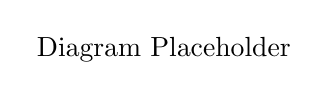
\begin{tikzpicture}
            %% Code for the actual diagram would go here. Replace the text with the corresponding TikZ commands.
            \node at (0, 0) {Diagram Placeholder};
        \end{tikzpicture}
    \end{center}
